BDT training and testing is executed with the Toolkit for Multivariate Data Analysis (TMVA), a customizable machine learning environment available in ROOT~\cite{TMVA}. Boosting is performed with the Gradient Boost algorithm, selected for its stability over other boosting methods (e.g., Adaptive Boost). 

A BDT was trained for each leptoquark mass point using the combined 2016, 2017, and 2018 background and signal MC datasets described in Section~\ref{sec:Backgrounds}. Samples have the same preselection, b-jet requirement, data and MC corrections, and background normalization scale factors applied as listed in Sections~\ref{sec:Preselection},~\ref{sec:Corrections}, and~\ref{sec:BkgNorm}. Two additional cuts are applied prior to training: one cut at $\Muu > \SI{250}{\GeV}$ to exclude events in the background normalization control regions and a signal-dependent cut at $\Muujj > \MLQ$, i.e., half of the \HepProcess{\LQ\LQbar} resonance mass, to remove events far below the signal region. This additional selection ensures the training data are not dominated by background events that could result in bias. Complementary training and testing datasets are created by randomly selecting events from MC in a way that forbids any overlap. Events selected for training are reweighted such that the effective number of events in both signal and background classes are equal. Events with negative weights are ignored in training, as negative weights are not handled well in TMVA (specifically when using Gradient Boost). 

A collection of 11 kinematic variables were selected as inputs to the BDT training for their ability to discriminate between signal and background: 
\begin{itemize}
    \item Invariant masses: \Muu, \Muujj, \MujOne, \MujTwo
    \item Particle momenta: \ptof{\PmuOne}, \ptof{\PmuTwo}, \ptof{\PjOne}, \ptof{\PjTwo}
    \item Combined momenta: \ST, \MET
    \item Spatial separation between the dimuon pair and the leading-\pt jet: \DRof{\PmuOne+\PmuTwo}{\PjOne}
\end{itemize}
Figures~\ref{figapp:variables1}--\ref{figapp:variables6} show the distribution of each variable in background and signal events. Linear correlations (Figs.~\ref{figapp:correlationsBkg1}--\ref{figapp:correlationsSig3}) between variables were studied alongside variable rankings to avoid including highly-correlated but low-ranking variables, which introduces information redundancy. A common risk when using Gradient Boost is overtraining, where the BDT is optimized to bias in the training samples, degrading its performance. To check for overtraining, the BDT response was compared between training and testing data using the Kolmogorov-Smirnov test; no overfitting was observed. Optimal performance of each BDT was verified by checking the area under the Receiver Operating Characteristic (ROC) curve, which plots background rejection vs. signal efficiency, shown in Figs.~\ref{figapp:roc1}--\ref{figapp:roc2}. Figures~\ref{figapp:overtraining1}--\ref{figapp:overtraining2} show the BDT response in training and testing data and the corresponding ROC curves.

\begin{figure}[H]
    \centering
    {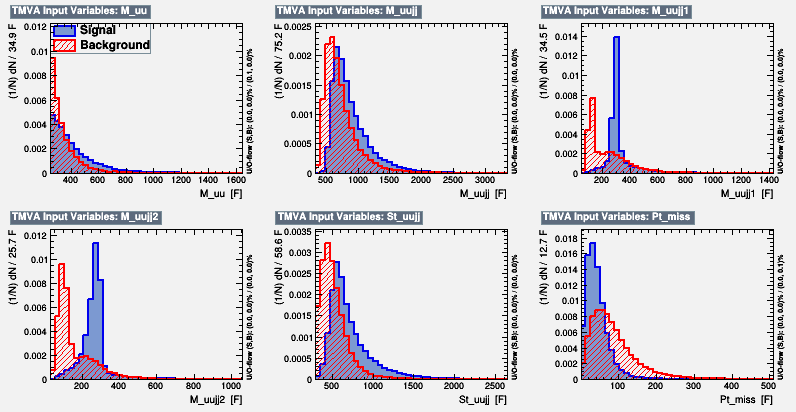
\includegraphics[width=.49\textwidth]{Images/Analysis/Results_LQToBMu_pair_uubj_BDTG_FullRun2_2023_01_25_020318/300/variables_id_c1.png}}
    {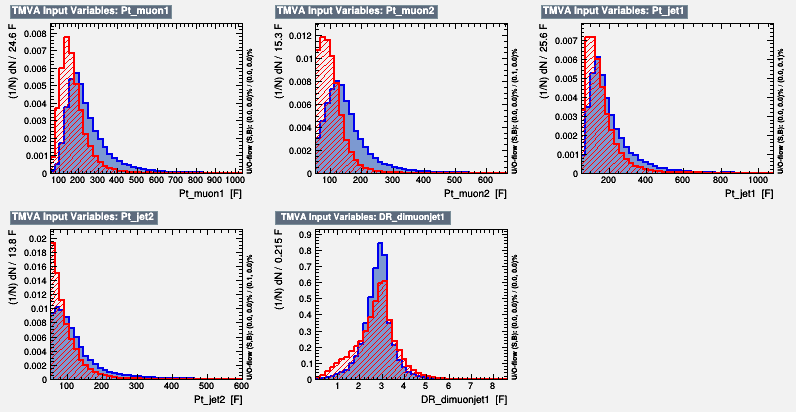
\includegraphics[width=.49\textwidth]{Images/Analysis/Results_LQToBMu_pair_uubj_BDTG_FullRun2_2023_01_25_020318/300/variables_id_c2.png}}
    {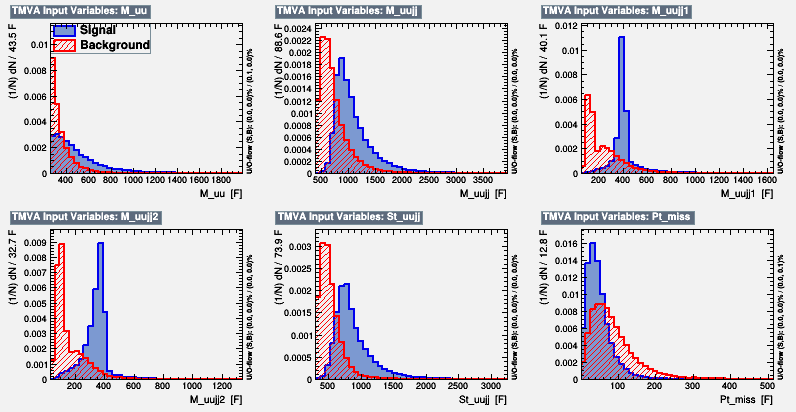
\includegraphics[width=.49\textwidth]{Images/Analysis/Results_LQToBMu_pair_uubj_BDTG_FullRun2_2023_01_25_020318/400/variables_id_c1.png}}
    {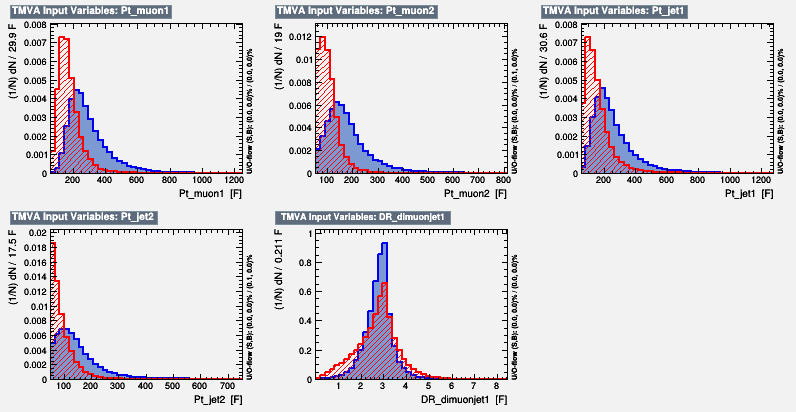
\includegraphics[width=.49\textwidth]{Images/Analysis/Results_LQToBMu_pair_uubj_BDTG_FullRun2_2023_01_25_020318/400/variables_id_c2.png}}
    {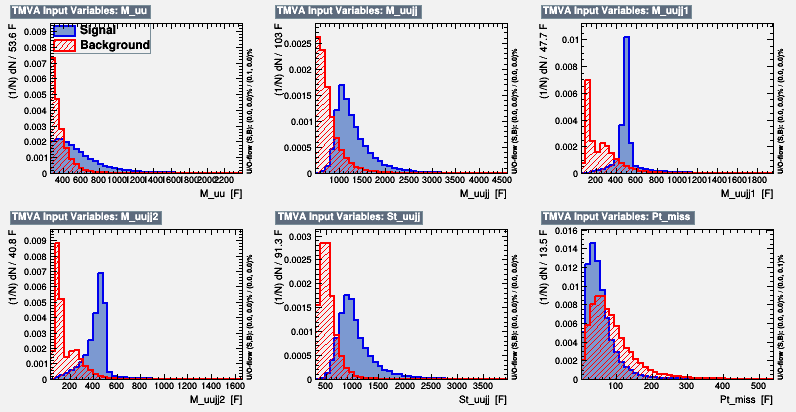
\includegraphics[width=.49\textwidth]{Images/Analysis/Results_LQToBMu_pair_uubj_BDTG_FullRun2_2023_01_25_020318/500/variables_id_c1.png}}
    {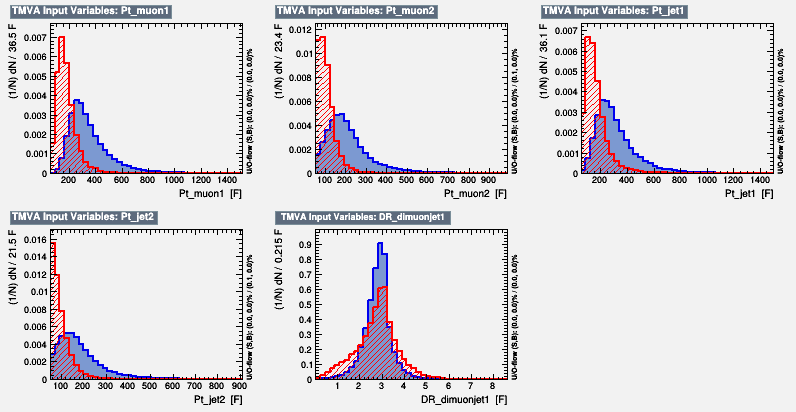
\includegraphics[width=.49\textwidth]{Images/Analysis/Results_LQToBMu_pair_uubj_BDTG_FullRun2_2023_01_25_020318/500/variables_id_c2.png}}
    {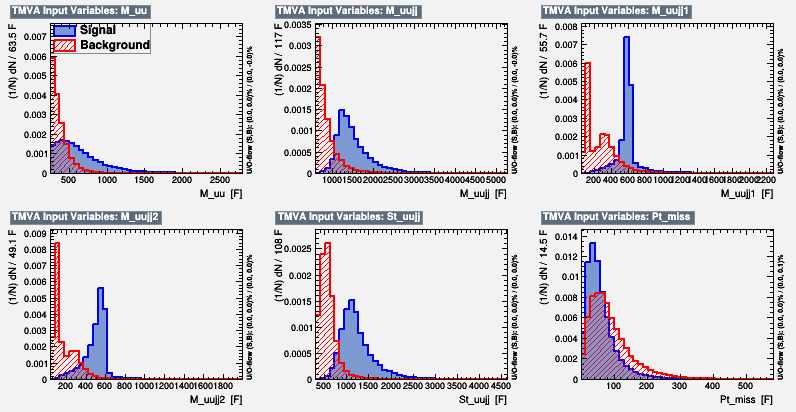
\includegraphics[width=.49\textwidth]{Images/Analysis/Results_LQToBMu_pair_uubj_BDTG_FullRun2_2023_01_25_020318/600/variables_id_c1.png}}
    {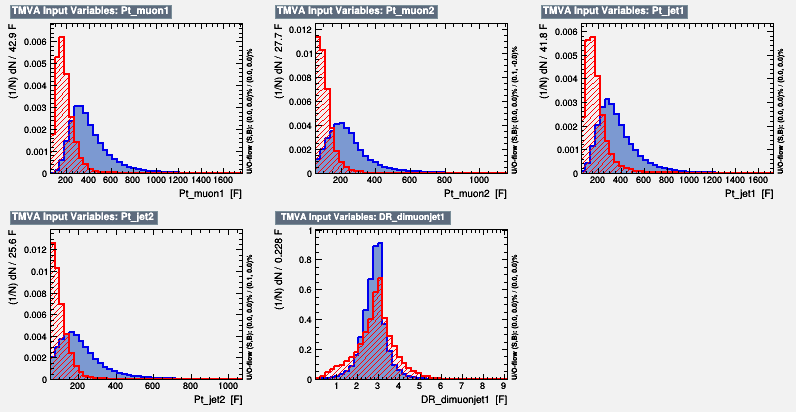
\includegraphics[width=.49\textwidth]{Images/Analysis/Results_LQToBMu_pair_uubj_BDTG_FullRun2_2023_01_25_020318/600/variables_id_c2.png}}
    {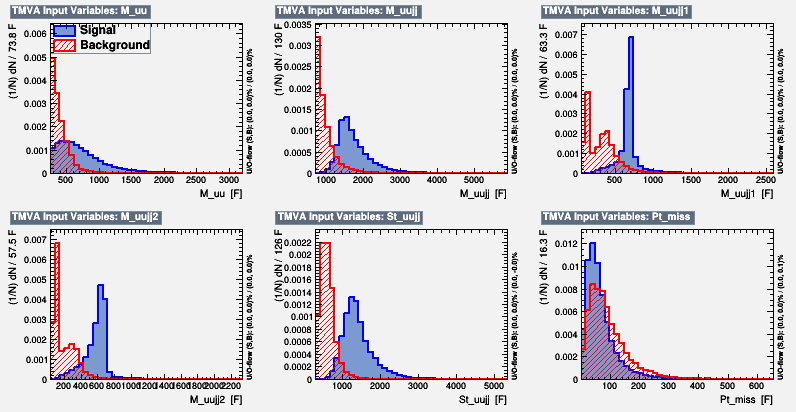
\includegraphics[width=.49\textwidth]{Images/Analysis/Results_LQToBMu_pair_uubj_BDTG_FullRun2_2023_01_25_020318/700/variables_id_c1.png}}
    {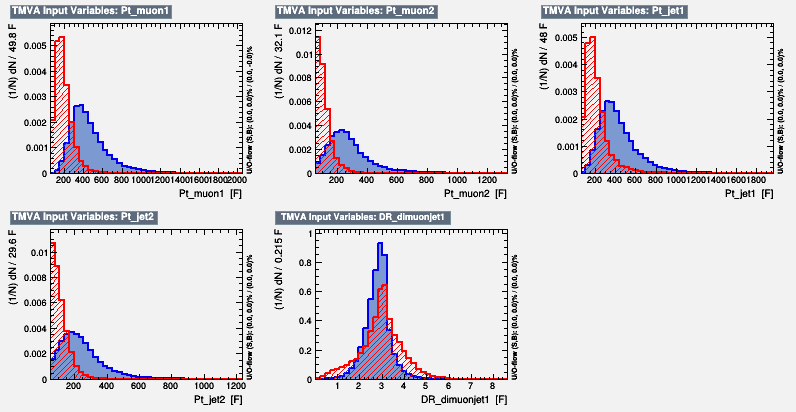
\includegraphics[width=.49\textwidth]{Images/Analysis/Results_LQToBMu_pair_uubj_BDTG_FullRun2_2023_01_25_020318/700/variables_id_c2.png}}
    \caption{A comparison between background and signal events in the BDT input variables corresponding to BDT trainings on 300 to \SI{700}{GeV} leptoquark signal samples. Signal events are solid blue while background events are hashed red.}
    \label{figapp:variables1}
\end{figure}

\begin{figure}[H]
    \centering
    {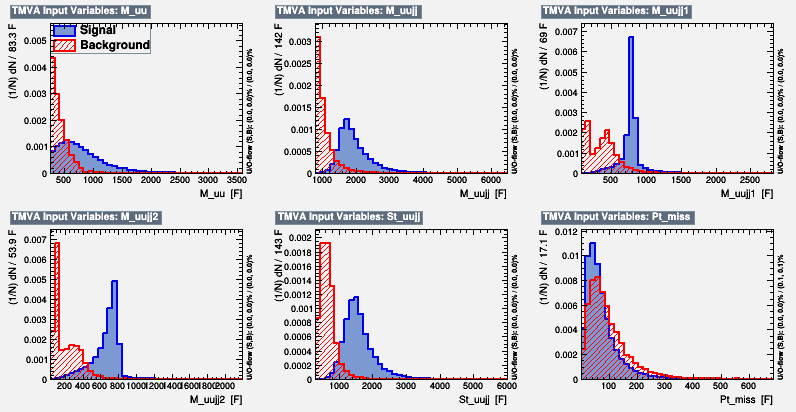
\includegraphics[width=.49\textwidth]{Images/Analysis/Results_LQToBMu_pair_uubj_BDTG_FullRun2_2023_01_25_020318/800/variables_id_c1.png}}
    {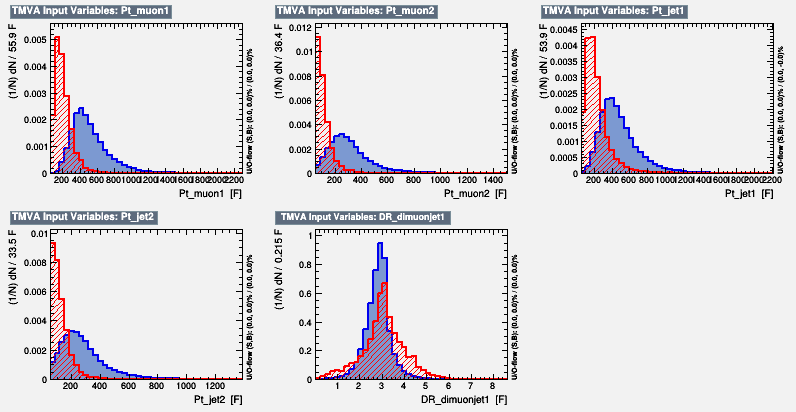
\includegraphics[width=.49\textwidth]{Images/Analysis/Results_LQToBMu_pair_uubj_BDTG_FullRun2_2023_01_25_020318/800/variables_id_c2.png}}
    {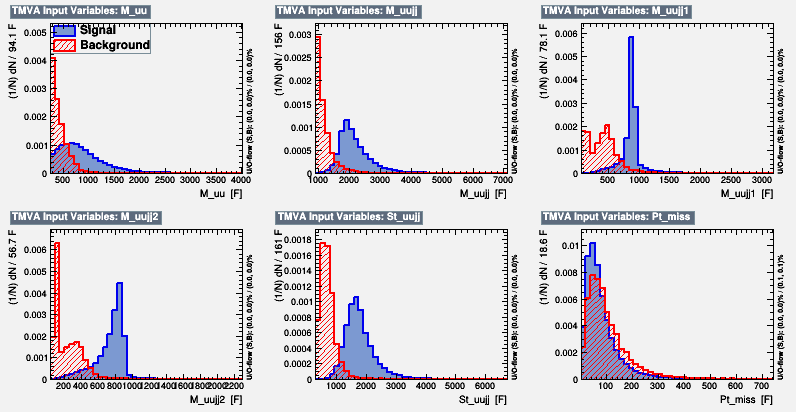
\includegraphics[width=.49\textwidth]{Images/Analysis/Results_LQToBMu_pair_uubj_BDTG_FullRun2_2023_01_25_020318/900/variables_id_c1.png}}
    {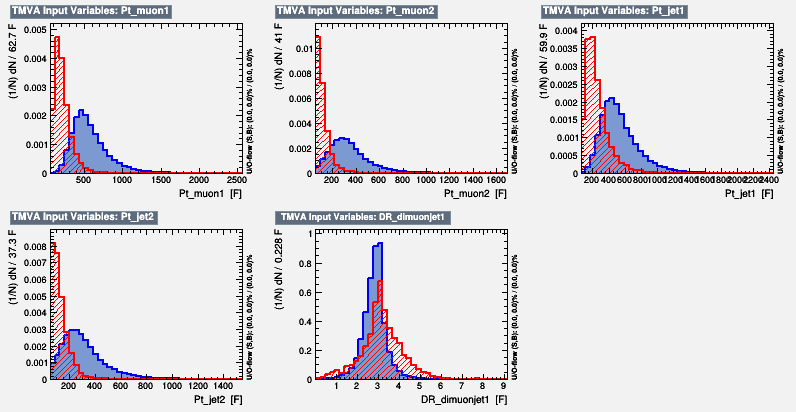
\includegraphics[width=.49\textwidth]{Images/Analysis/Results_LQToBMu_pair_uubj_BDTG_FullRun2_2023_01_25_020318/900/variables_id_c2.png}}
    {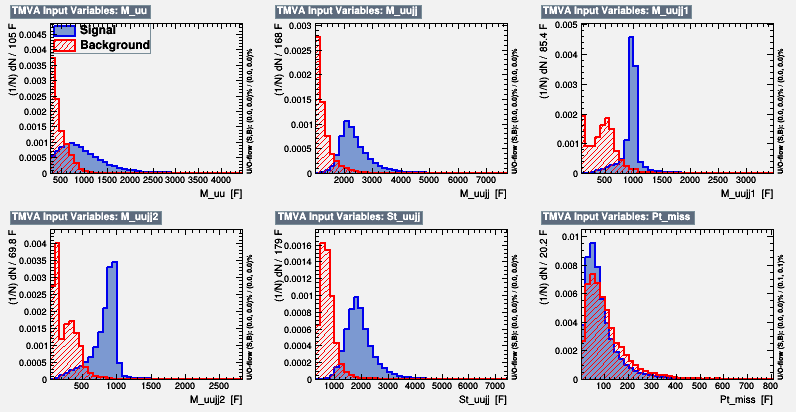
\includegraphics[width=.49\textwidth]{Images/Analysis/Results_LQToBMu_pair_uubj_BDTG_FullRun2_2023_01_25_020318/1000/variables_id_c1.png}}
    {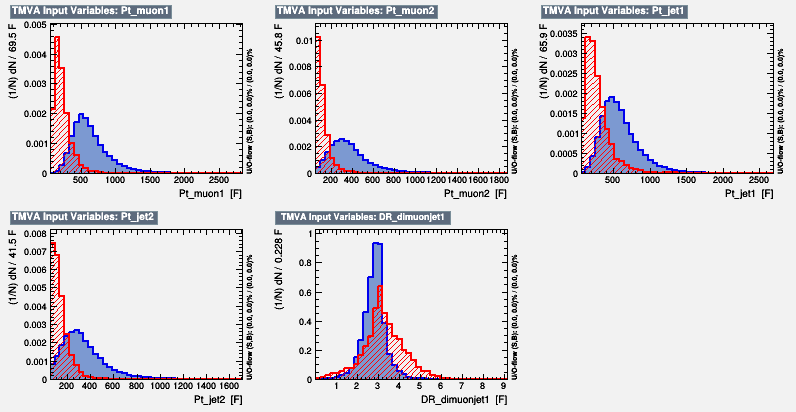
\includegraphics[width=.49\textwidth]{Images/Analysis/Results_LQToBMu_pair_uubj_BDTG_FullRun2_2023_01_25_020318/1000/variables_id_c2.png}}
    {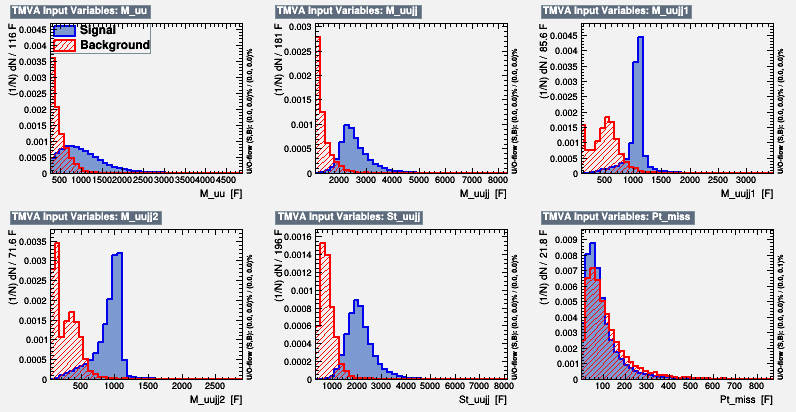
\includegraphics[width=.49\textwidth]{Images/Analysis/Results_LQToBMu_pair_uubj_BDTG_FullRun2_2023_01_25_020318/1100/variables_id_c1.png}}
    {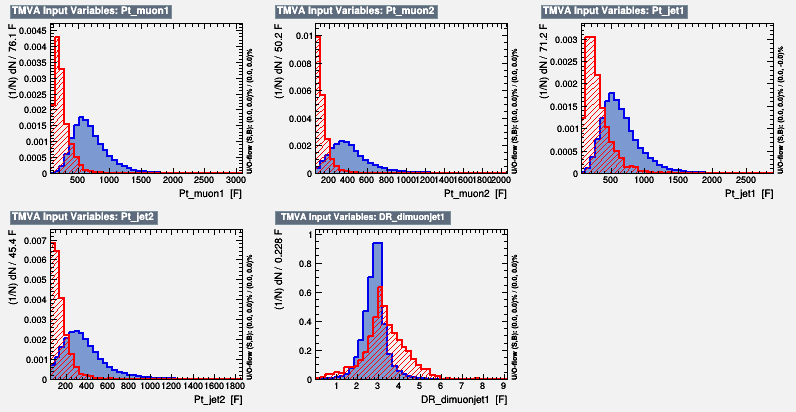
\includegraphics[width=.49\textwidth]{Images/Analysis/Results_LQToBMu_pair_uubj_BDTG_FullRun2_2023_01_25_020318/1100/variables_id_c2.png}}
    {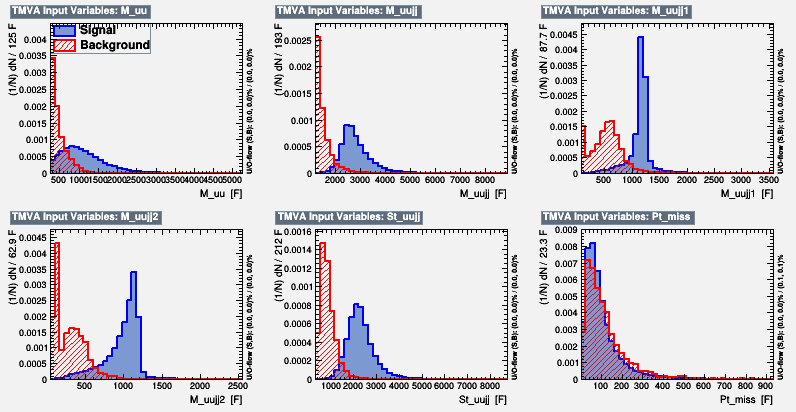
\includegraphics[width=.49\textwidth]{Images/Analysis/Results_LQToBMu_pair_uubj_BDTG_FullRun2_2023_01_25_020318/1200/variables_id_c1.png}}
    {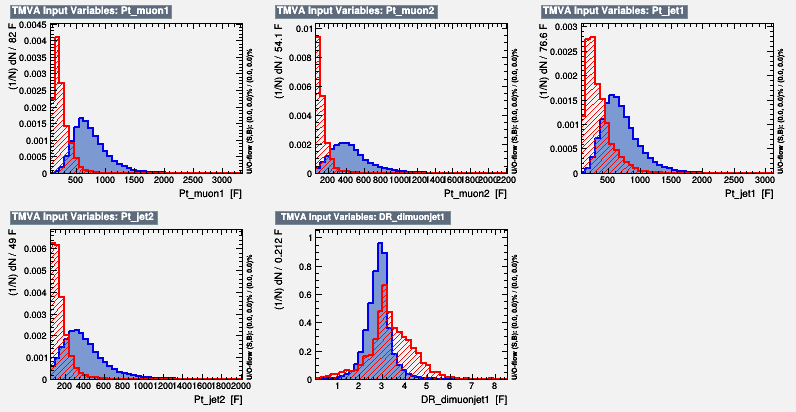
\includegraphics[width=.49\textwidth]{Images/Analysis/Results_LQToBMu_pair_uubj_BDTG_FullRun2_2023_01_25_020318/1200/variables_id_c2.png}}
    \caption{A comparison between background and signal events in the BDT input variables corresponding to BDT trainings on 800 to \SI{1200}{GeV} leptoquark signal samples. Signal events are solid blue while background events are hashed red.}
    \label{figapp:variables2}
\end{figure}

\begin{figure}[H]
    \centering
    {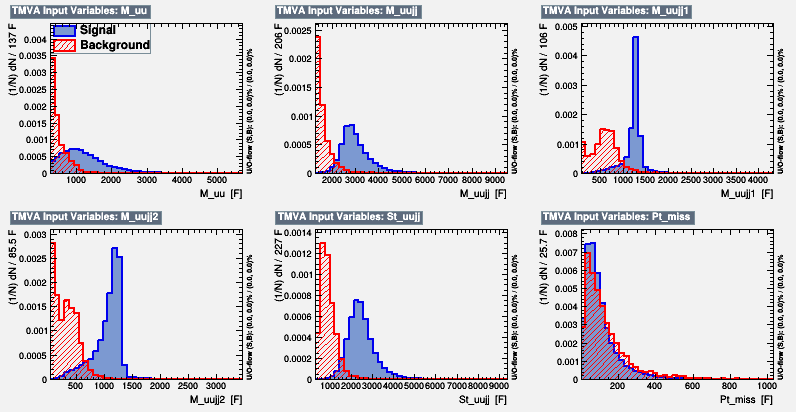
\includegraphics[width=.49\textwidth]{Images/Analysis/Results_LQToBMu_pair_uubj_BDTG_FullRun2_2023_01_25_020318/1300/variables_id_c1.png}}
    {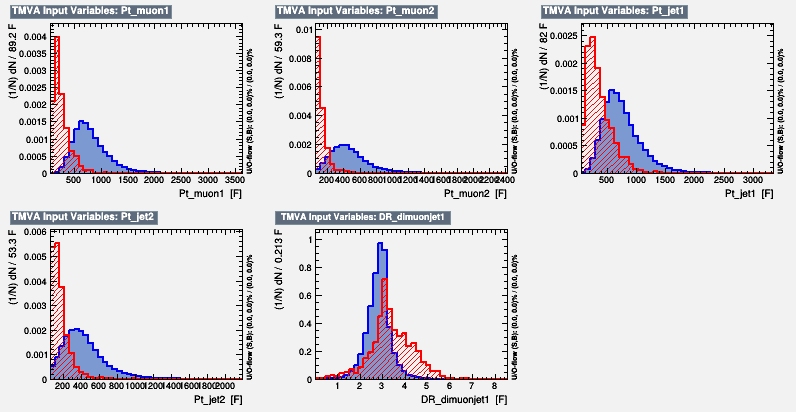
\includegraphics[width=.49\textwidth]{Images/Analysis/Results_LQToBMu_pair_uubj_BDTG_FullRun2_2023_01_25_020318/1300/variables_id_c2.png}}
    {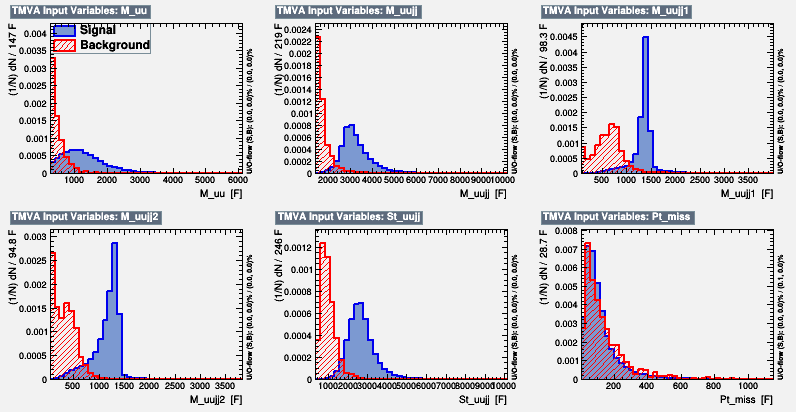
\includegraphics[width=.49\textwidth]{Images/Analysis/Results_LQToBMu_pair_uubj_BDTG_FullRun2_2023_01_25_020318/1400/variables_id_c1.png}}
    {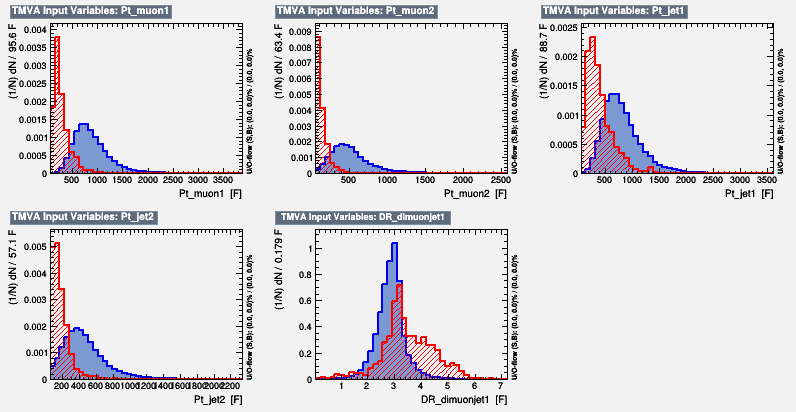
\includegraphics[width=.49\textwidth]{Images/Analysis/Results_LQToBMu_pair_uubj_BDTG_FullRun2_2023_01_25_020318/1400/variables_id_c2.png}}
    {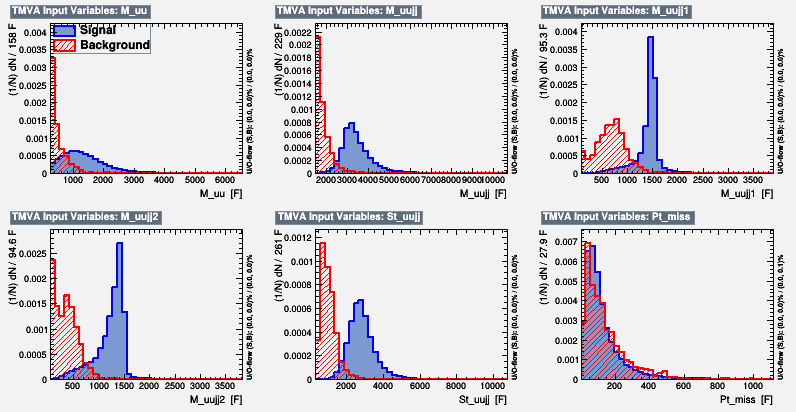
\includegraphics[width=.49\textwidth]{Images/Analysis/Results_LQToBMu_pair_uubj_BDTG_FullRun2_2023_01_25_020318/1500/variables_id_c1.png}}
    {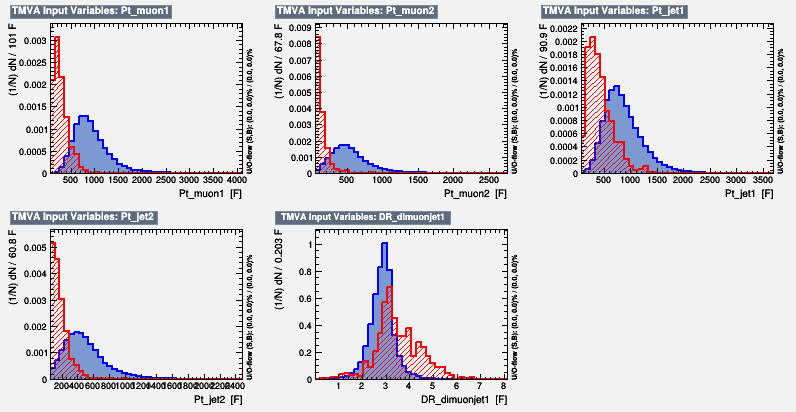
\includegraphics[width=.49\textwidth]{Images/Analysis/Results_LQToBMu_pair_uubj_BDTG_FullRun2_2023_01_25_020318/1500/variables_id_c2.png}}
    {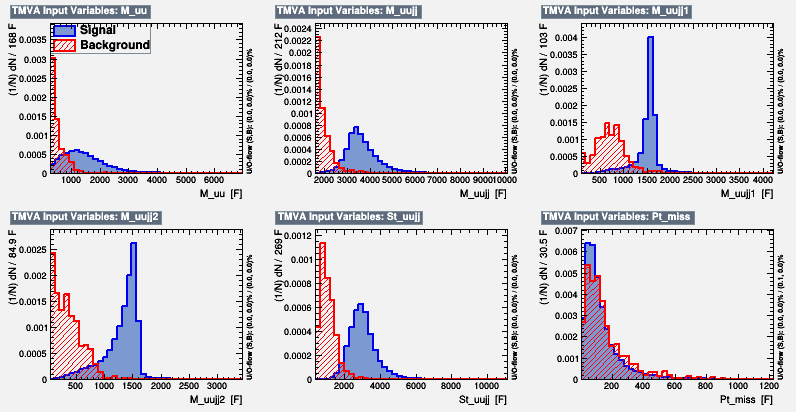
\includegraphics[width=.49\textwidth]{Images/Analysis/Results_LQToBMu_pair_uubj_BDTG_FullRun2_2023_01_25_020318/1600/variables_id_c1.png}}
    {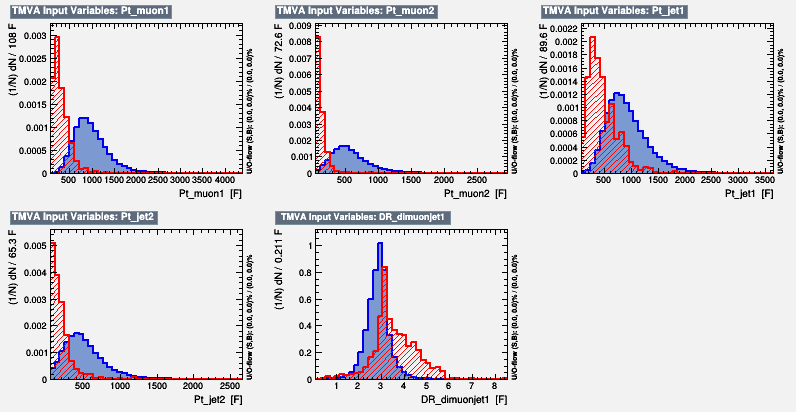
\includegraphics[width=.49\textwidth]{Images/Analysis/Results_LQToBMu_pair_uubj_BDTG_FullRun2_2023_01_25_020318/1600/variables_id_c2.png}}
    {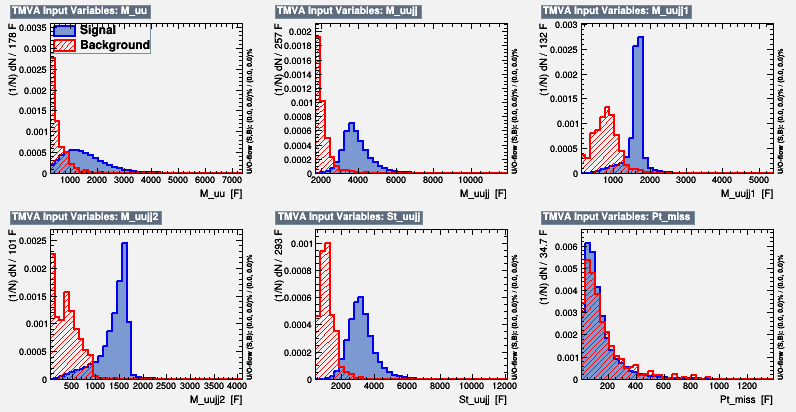
\includegraphics[width=.49\textwidth]{Images/Analysis/Results_LQToBMu_pair_uubj_BDTG_FullRun2_2023_01_25_020318/1700/variables_id_c1.png}}
    {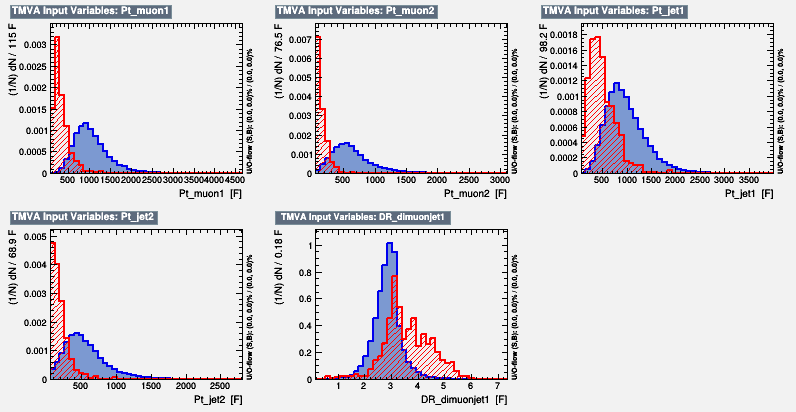
\includegraphics[width=.49\textwidth]{Images/Analysis/Results_LQToBMu_pair_uubj_BDTG_FullRun2_2023_01_25_020318/1700/variables_id_c2.png}}
    \caption{A comparison between background and signal events in the BDT input variables corresponding to BDT trainings on 1300 to \SI{1700}{GeV} leptoquark signal samples. Signal events are solid blue while background events are hashed red.}
    \label{figapp:variables3}
\end{figure}

\begin{figure}[H]
    \centering
    {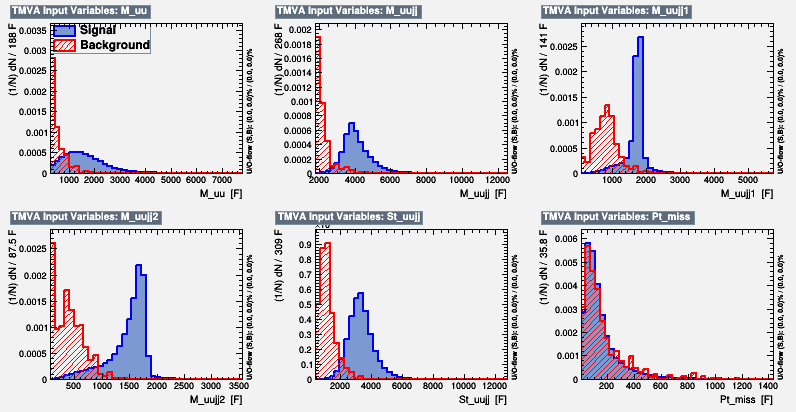
\includegraphics[width=.49\textwidth]{Images/Analysis/Results_LQToBMu_pair_uubj_BDTG_FullRun2_2023_01_25_020318/1800/variables_id_c1.png}}
    {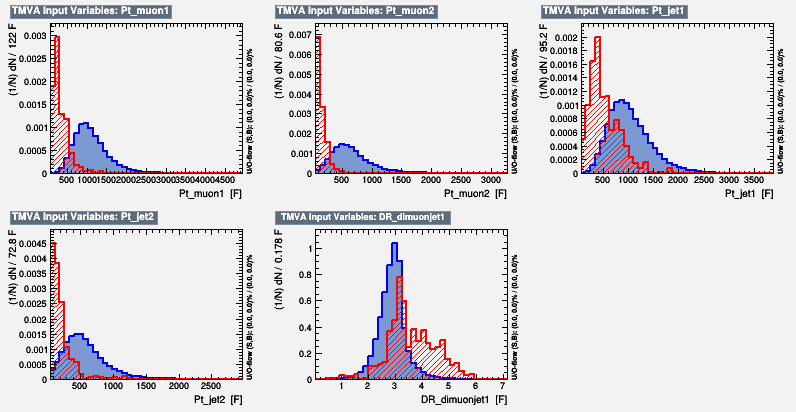
\includegraphics[width=.49\textwidth]{Images/Analysis/Results_LQToBMu_pair_uubj_BDTG_FullRun2_2023_01_25_020318/1800/variables_id_c2.png}}
    {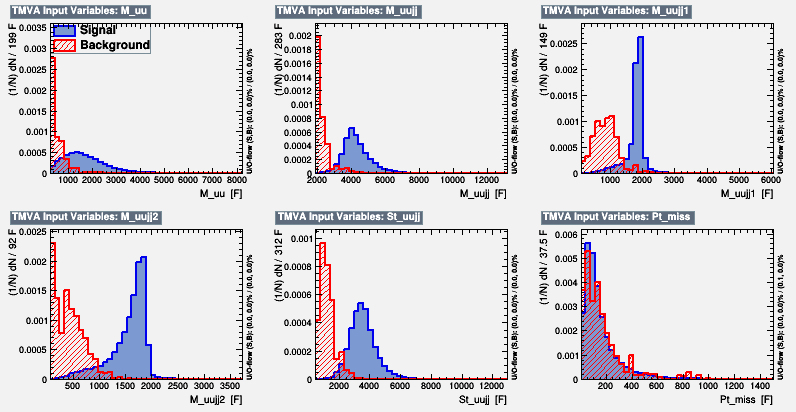
\includegraphics[width=.49\textwidth]{Images/Analysis/Results_LQToBMu_pair_uubj_BDTG_FullRun2_2023_01_25_020318/1900/variables_id_c1.png}}
    {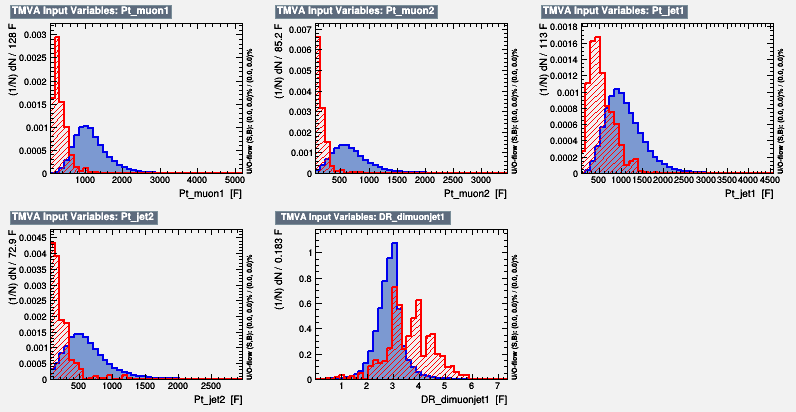
\includegraphics[width=.49\textwidth]{Images/Analysis/Results_LQToBMu_pair_uubj_BDTG_FullRun2_2023_01_25_020318/1900/variables_id_c2.png}}
    {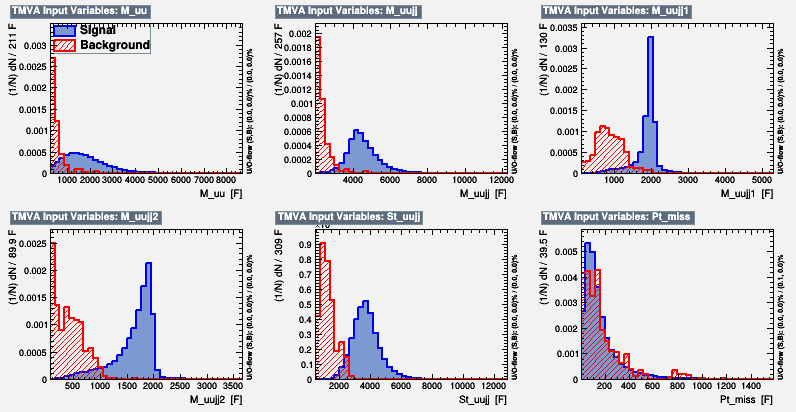
\includegraphics[width=.49\textwidth]{Images/Analysis/Results_LQToBMu_pair_uubj_BDTG_FullRun2_2023_01_25_020318/2000/variables_id_c1.png}}
    {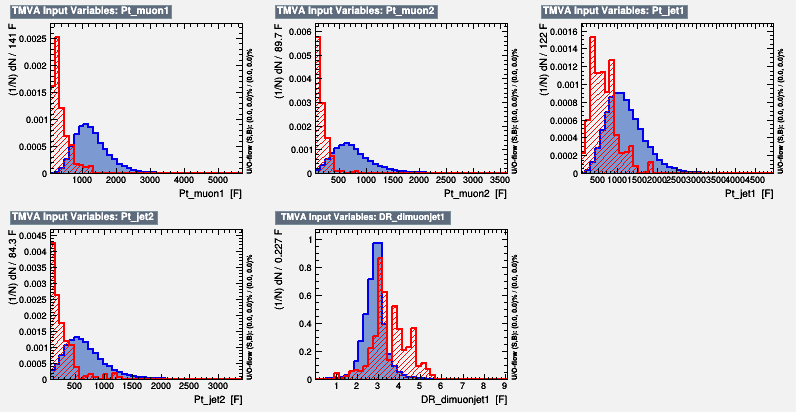
\includegraphics[width=.49\textwidth]{Images/Analysis/Results_LQToBMu_pair_uubj_BDTG_FullRun2_2023_01_25_020318/2100/variables_id_c2.png}}
    {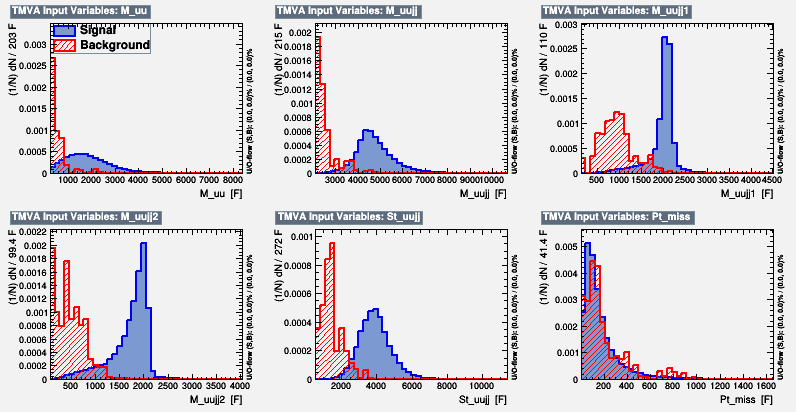
\includegraphics[width=.49\textwidth]{Images/Analysis/Results_LQToBMu_pair_uubj_BDTG_FullRun2_2023_01_25_020318/2100/variables_id_c1.png}}
    {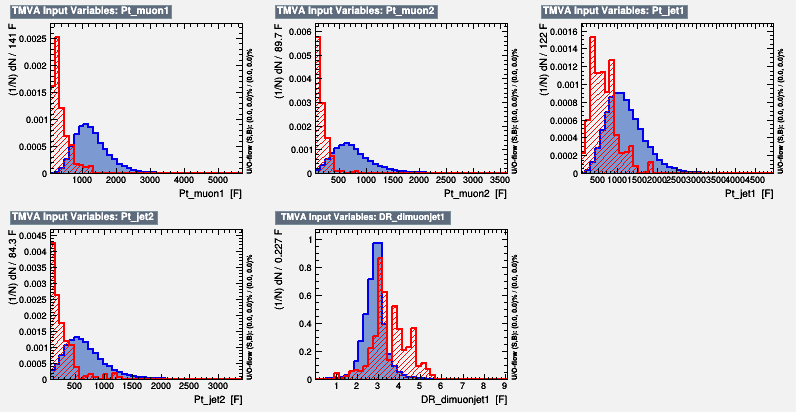
\includegraphics[width=.49\textwidth]{Images/Analysis/Results_LQToBMu_pair_uubj_BDTG_FullRun2_2023_01_25_020318/2100/variables_id_c2.png}}
    {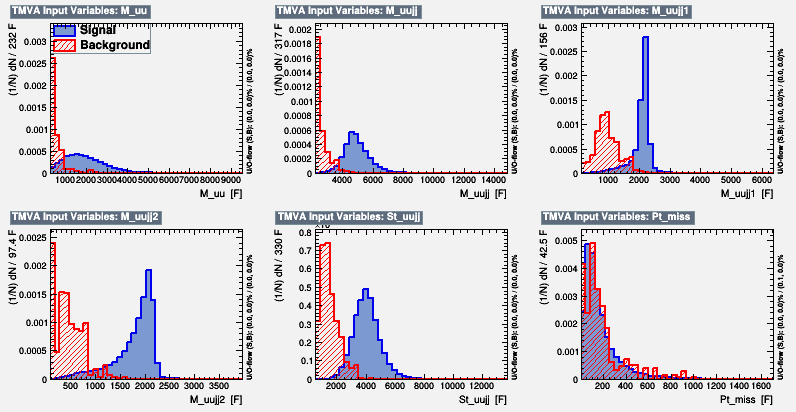
\includegraphics[width=.49\textwidth]{Images/Analysis/Results_LQToBMu_pair_uubj_BDTG_FullRun2_2023_01_25_020318/2200/variables_id_c1.png}}
    {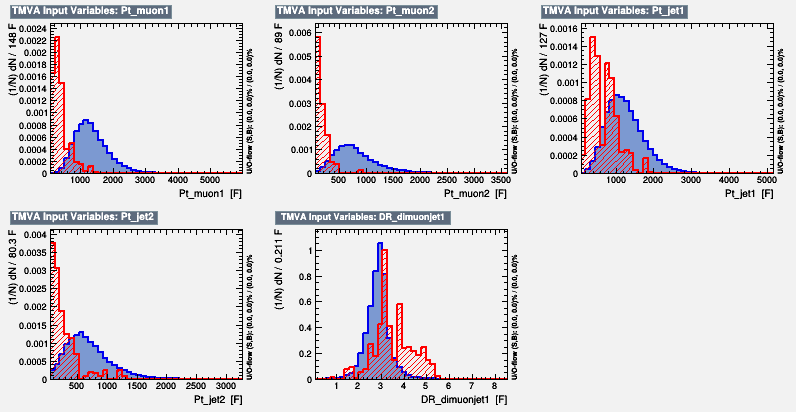
\includegraphics[width=.49\textwidth]{Images/Analysis/Results_LQToBMu_pair_uubj_BDTG_FullRun2_2023_01_25_020318/2200/variables_id_c2.png}}
    \caption{A comparison between background and events in the BDT input variables corresponding to BDT trainings on 1800 to \SI{2200}{GeV} leptoquark signal samples. Signal events are solid blue while background events are hashed red.}
    \label{figapp:variables4}
\end{figure}

\begin{figure}[H]
    \centering
    {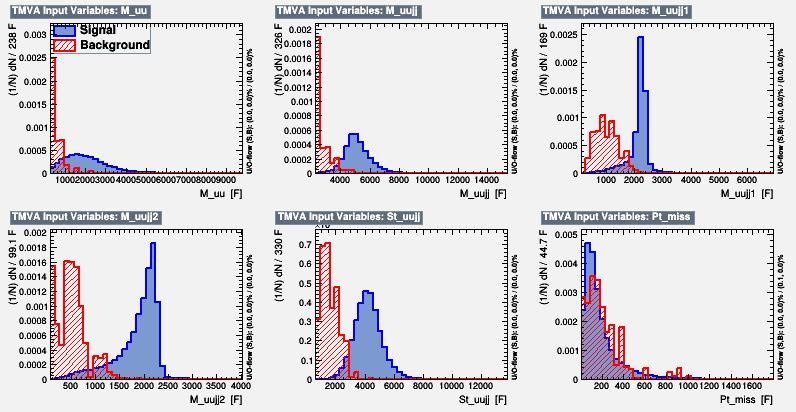
\includegraphics[width=.49\textwidth]{Images/Analysis/Results_LQToBMu_pair_uubj_BDTG_FullRun2_2023_01_25_020318/2300/variables_id_c1.png}}
    {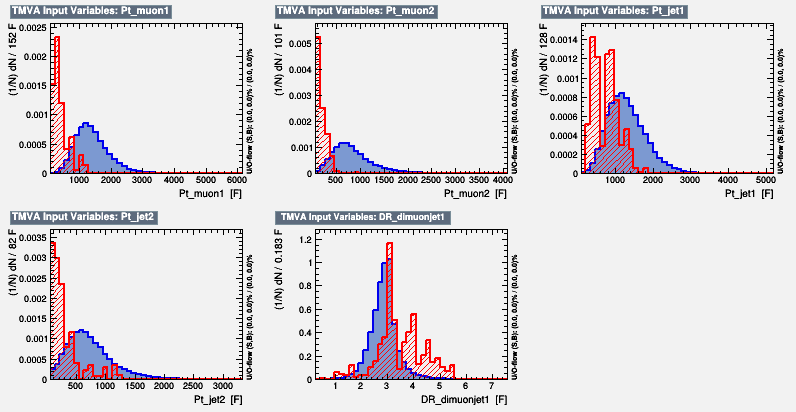
\includegraphics[width=.49\textwidth]{Images/Analysis/Results_LQToBMu_pair_uubj_BDTG_FullRun2_2023_01_25_020318/2300/variables_id_c2.png}}
    {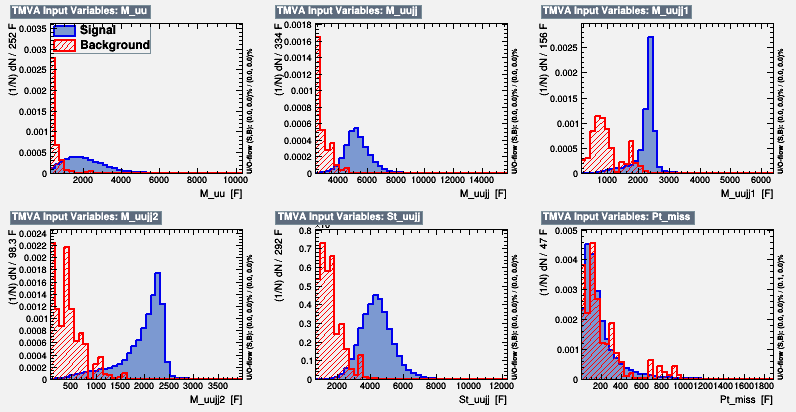
\includegraphics[width=.49\textwidth]{Images/Analysis/Results_LQToBMu_pair_uubj_BDTG_FullRun2_2023_01_25_020318/2400/variables_id_c1.png}}
    {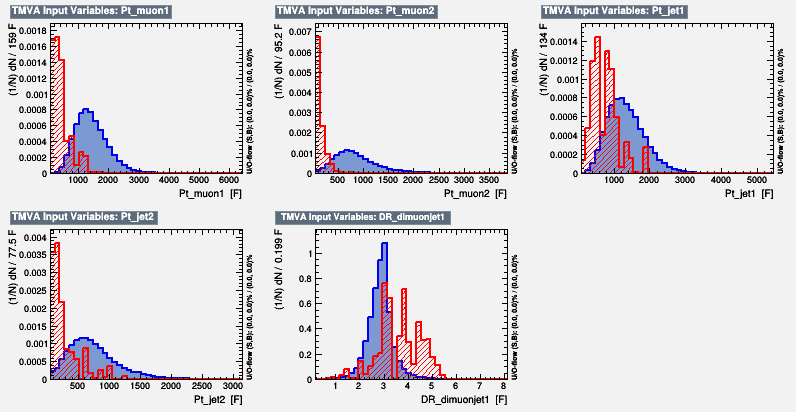
\includegraphics[width=.49\textwidth]{Images/Analysis/Results_LQToBMu_pair_uubj_BDTG_FullRun2_2023_01_25_020318/2400/variables_id_c2.png}}
    {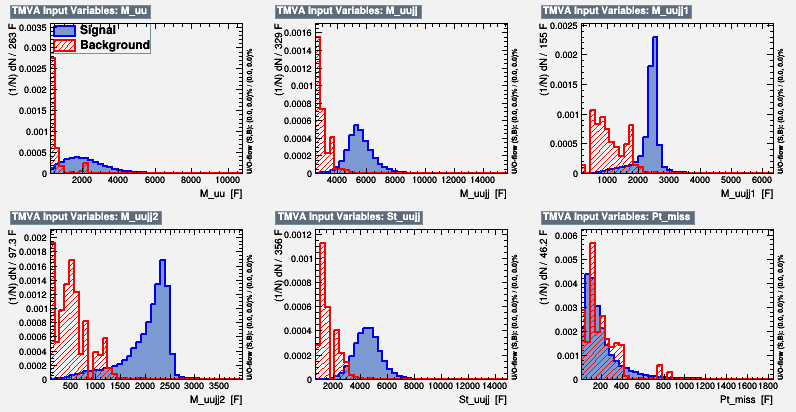
\includegraphics[width=.49\textwidth]{Images/Analysis/Results_LQToBMu_pair_uubj_BDTG_FullRun2_2023_01_25_020318/2500/variables_id_c1.png}}
    {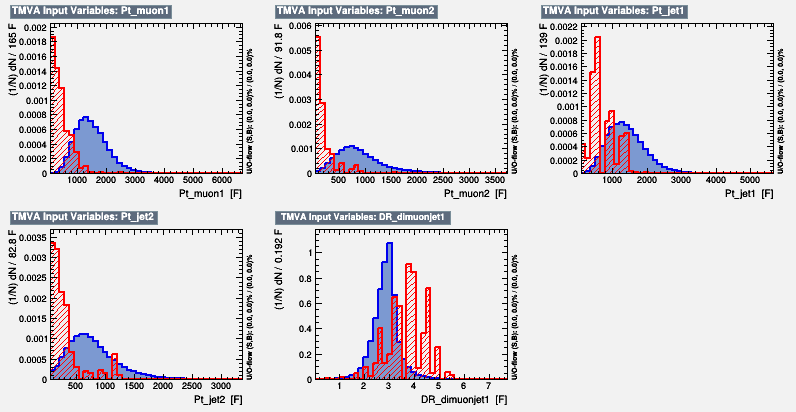
\includegraphics[width=.49\textwidth]{Images/Analysis/Results_LQToBMu_pair_uubj_BDTG_FullRun2_2023_01_25_020318/2500/variables_id_c2.png}}
    {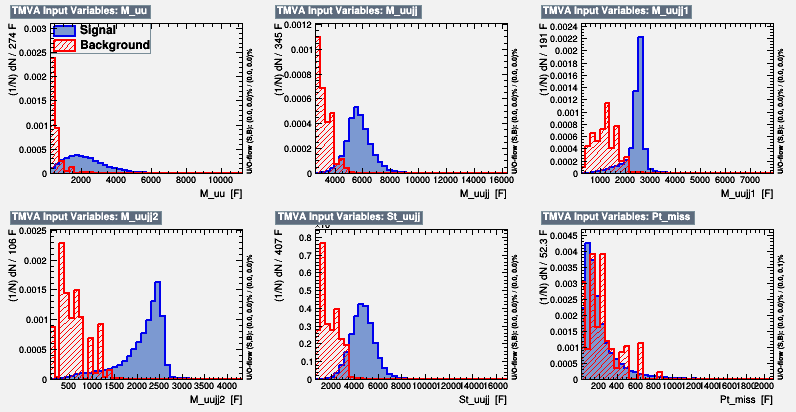
\includegraphics[width=.49\textwidth]{Images/Analysis/Results_LQToBMu_pair_uubj_BDTG_FullRun2_2023_01_25_020318/2600/variables_id_c1.png}}
    {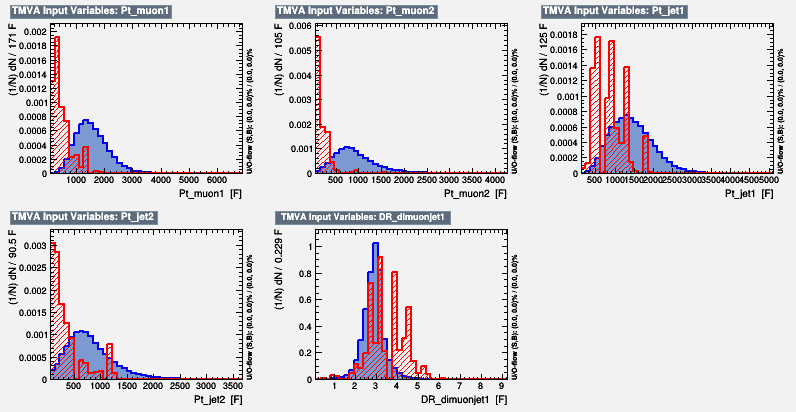
\includegraphics[width=.49\textwidth]{Images/Analysis/Results_LQToBMu_pair_uubj_BDTG_FullRun2_2023_01_25_020318/2600/variables_id_c2.png}}
    {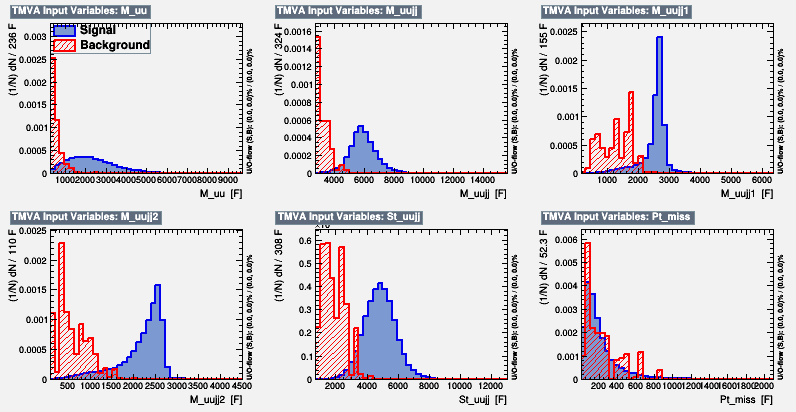
\includegraphics[width=.49\textwidth]{Images/Analysis/Results_LQToBMu_pair_uubj_BDTG_FullRun2_2023_01_25_020318/2700/variables_id_c1.png}}
    {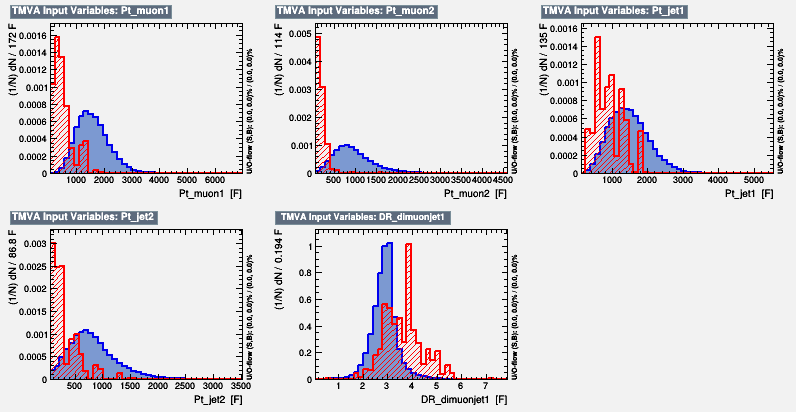
\includegraphics[width=.49\textwidth]{Images/Analysis/Results_LQToBMu_pair_uubj_BDTG_FullRun2_2023_01_25_020318/2700/variables_id_c2.png}}
    \caption{A comparison between background and signal events in the BDT input variables corresponding to BDT trainings on 2300 to \SI{2700}{GeV} leptoquark signal samples. Signal events are solid blue while background events are hashed red.}
    \label{figapp:variables5}
\end{figure}

\begin{figure}[H]
    \centering
    {\includegraphics[width=.49\textwidth]{Images/Analysis/Results_LQToBMu_pair_uubj_BDTG_FullRun2_2023_01_25_020318/2800/variables_id_c1.png}}
    {\includegraphics[width=.49\textwidth]{Images/Analysis/Results_LQToBMu_pair_uubj_BDTG_FullRun2_2023_01_25_020318/2800/variables_id_c2.png}}
    {\includegraphics[width=.49\textwidth]{Images/Analysis/Results_LQToBMu_pair_uubj_BDTG_FullRun2_2023_01_25_020318/2900/variables_id_c1.png}}
    {\includegraphics[width=.49\textwidth]{Images/Analysis/Results_LQToBMu_pair_uubj_BDTG_FullRun2_2023_01_25_020318/2900/variables_id_c2.png}}
    {\includegraphics[width=.49\textwidth]{Images/Analysis/Results_LQToBMu_pair_uubj_BDTG_FullRun2_2023_01_25_020318/3000/variables_id_c1.png}}
    {\includegraphics[width=.49\textwidth]{Images/Analysis/Results_LQToBMu_pair_uubj_BDTG_FullRun2_2023_01_25_020318/3000/variables_id_c2.png}}
    {\includegraphics[width=.49\textwidth]{Images/Analysis/Results_LQToBMu_pair_uubj_BDTG_FullRun2_2023_01_25_020318/3500/variables_id_c1.png}}
    {\includegraphics[width=.49\textwidth]{Images/Analysis/Results_LQToBMu_pair_uubj_BDTG_FullRun2_2023_01_25_020318/3500/variables_id_c2.png}}
    {\includegraphics[width=.49\textwidth]{Images/Analysis/Results_LQToBMu_pair_uubj_BDTG_FullRun2_2023_01_25_020318/4000/variables_id_c1.png}}
    {\includegraphics[width=.49\textwidth]{Images/Analysis/Results_LQToBMu_pair_uubj_BDTG_FullRun2_2023_01_25_020318/4000/variables_id_c2.png}}
    \caption{A comparison between background and signal events in the BDT input variables corresponding to BDT trainings on 2800 to \SI{4000}{GeV} leptoquark signal samples. Signal events are solid blue while background events are hashed red.}
    \label{figapp:variables6}
\end{figure}

\begin{figure}[H]
    \centering
    {\includegraphics[width=.30\textwidth]{Images/Analysis/Results_LQToBMu_pair_uubj_BDTG_FullRun2_2023_01_25_020318/300/CorrelationMatrixB.png}}
    {\includegraphics[width=.30\textwidth]{Images/Analysis/Results_LQToBMu_pair_uubj_BDTG_FullRun2_2023_01_25_020318/400/CorrelationMatrixB.png}}
    {\includegraphics[width=.30\textwidth]{Images/Analysis/Results_LQToBMu_pair_uubj_BDTG_FullRun2_2023_01_25_020318/500/CorrelationMatrixB.png}}
    {\includegraphics[width=.30\textwidth]{Images/Analysis/Results_LQToBMu_pair_uubj_BDTG_FullRun2_2023_01_25_020318/600/CorrelationMatrixB.png}}
    {\includegraphics[width=.30\textwidth]{Images/Analysis/Results_LQToBMu_pair_uubj_BDTG_FullRun2_2023_01_25_020318/700/CorrelationMatrixB.png}}
    {\includegraphics[width=.30\textwidth]{Images/Analysis/Results_LQToBMu_pair_uubj_BDTG_FullRun2_2023_01_25_020318/800/CorrelationMatrixB.png}}
    {\includegraphics[width=.30\textwidth]{Images/Analysis/Results_LQToBMu_pair_uubj_BDTG_FullRun2_2023_01_25_020318/900/CorrelationMatrixB.png}}
    {\includegraphics[width=.30\textwidth]{Images/Analysis/Results_LQToBMu_pair_uubj_BDTG_FullRun2_2023_01_25_020318/1000/CorrelationMatrixB.png}}
    {\includegraphics[width=.30\textwidth]{Images/Analysis/Results_LQToBMu_pair_uubj_BDTG_FullRun2_2023_01_25_020318/1100/CorrelationMatrixB.png}}
    {\includegraphics[width=.30\textwidth]{Images/Analysis/Results_LQToBMu_pair_uubj_BDTG_FullRun2_2023_01_25_020318/1200/CorrelationMatrixB.png}}
    {\includegraphics[width=.30\textwidth]{Images/Analysis/Results_LQToBMu_pair_uubj_BDTG_FullRun2_2023_01_25_020318/1300/CorrelationMatrixB.png}}
    {\includegraphics[width=.30\textwidth]{Images/Analysis/Results_LQToBMu_pair_uubj_BDTG_FullRun2_2023_01_25_020318/1400/CorrelationMatrixB.png}}
    \caption{The linear correlation matricies of BDT input variables in background events corresponding to BDT trainings on 300 to \SI{1400}{GeV} leptoquark signal samples.}
    \label{figapp:correlationsBkg1}
\end{figure}

\begin{figure}[H]
    \centering
    {\includegraphics[width=.30\textwidth]{Images/Analysis/Results_LQToBMu_pair_uubj_BDTG_FullRun2_2023_01_25_020318/1500/CorrelationMatrixB.png}}
    {\includegraphics[width=.30\textwidth]{Images/Analysis/Results_LQToBMu_pair_uubj_BDTG_FullRun2_2023_01_25_020318/1600/CorrelationMatrixB.png}}
    {\includegraphics[width=.30\textwidth]{Images/Analysis/Results_LQToBMu_pair_uubj_BDTG_FullRun2_2023_01_25_020318/1700/CorrelationMatrixB.png}}
    {\includegraphics[width=.30\textwidth]{Images/Analysis/Results_LQToBMu_pair_uubj_BDTG_FullRun2_2023_01_25_020318/1800/CorrelationMatrixB.png}}
    {\includegraphics[width=.30\textwidth]{Images/Analysis/Results_LQToBMu_pair_uubj_BDTG_FullRun2_2023_01_25_020318/1900/CorrelationMatrixB.png}}
    {\includegraphics[width=.30\textwidth]{Images/Analysis/Results_LQToBMu_pair_uubj_BDTG_FullRun2_2023_01_25_020318/2000/CorrelationMatrixB.png}}
    {\includegraphics[width=.30\textwidth]{Images/Analysis/Results_LQToBMu_pair_uubj_BDTG_FullRun2_2023_01_25_020318/2100/CorrelationMatrixB.png}}
    {\includegraphics[width=.30\textwidth]{Images/Analysis/Results_LQToBMu_pair_uubj_BDTG_FullRun2_2023_01_25_020318/2200/CorrelationMatrixB.png}}
    {\includegraphics[width=.30\textwidth]{Images/Analysis/Results_LQToBMu_pair_uubj_BDTG_FullRun2_2023_01_25_020318/2300/CorrelationMatrixB.png}}
    {\includegraphics[width=.30\textwidth]{Images/Analysis/Results_LQToBMu_pair_uubj_BDTG_FullRun2_2023_01_25_020318/2400/CorrelationMatrixB.png}}
    {\includegraphics[width=.30\textwidth]{Images/Analysis/Results_LQToBMu_pair_uubj_BDTG_FullRun2_2023_01_25_020318/2500/CorrelationMatrixB.png}}
    {\includegraphics[width=.30\textwidth]{Images/Analysis/Results_LQToBMu_pair_uubj_BDTG_FullRun2_2023_01_25_020318/2600/CorrelationMatrixB.png}}
    \caption{The linear correlation matricies of BDT input variables in background events corresponding to BDT trainings on 1500 to \SI{2600}{GeV} leptoquark signal samples.}
    \label{figapp:correlationsBkg2}
\end{figure}

\begin{figure}[H]
    \centering
    {\includegraphics[width=.30\textwidth]{Images/Analysis/Results_LQToBMu_pair_uubj_BDTG_FullRun2_2023_01_25_020318/2700/CorrelationMatrixB.png}}
    {\includegraphics[width=.30\textwidth]{Images/Analysis/Results_LQToBMu_pair_uubj_BDTG_FullRun2_2023_01_25_020318/2800/CorrelationMatrixB.png}}
    {\includegraphics[width=.30\textwidth]{Images/Analysis/Results_LQToBMu_pair_uubj_BDTG_FullRun2_2023_01_25_020318/2900/CorrelationMatrixB.png}}
    {\includegraphics[width=.30\textwidth]{Images/Analysis/Results_LQToBMu_pair_uubj_BDTG_FullRun2_2023_01_25_020318/3000/CorrelationMatrixB.png}}
    {\includegraphics[width=.30\textwidth]{Images/Analysis/Results_LQToBMu_pair_uubj_BDTG_FullRun2_2023_01_25_020318/3500/CorrelationMatrixB.png}}
    {\includegraphics[width=.30\textwidth]{Images/Analysis/Results_LQToBMu_pair_uubj_BDTG_FullRun2_2023_01_25_020318/4000/CorrelationMatrixB.png}}
    \caption{The linear correlation matricies of BDT input variables in background events corresponding to BDT trainings on 2700 to \SI{4000}{GeV} leptoquark signal samples.}
    \label{figapp:correlationsBkg3}
\end{figure}

\begin{figure}[H]
    \centering
    {\includegraphics[width=.30\textwidth]{Images/Analysis/Results_LQToBMu_pair_uubj_BDTG_FullRun2_2023_01_25_020318/300/CorrelationMatrixS.png}}
    {\includegraphics[width=.30\textwidth]{Images/Analysis/Results_LQToBMu_pair_uubj_BDTG_FullRun2_2023_01_25_020318/400/CorrelationMatrixS.png}}
    {\includegraphics[width=.30\textwidth]{Images/Analysis/Results_LQToBMu_pair_uubj_BDTG_FullRun2_2023_01_25_020318/500/CorrelationMatrixS.png}}
    {\includegraphics[width=.30\textwidth]{Images/Analysis/Results_LQToBMu_pair_uubj_BDTG_FullRun2_2023_01_25_020318/600/CorrelationMatrixS.png}}
    {\includegraphics[width=.30\textwidth]{Images/Analysis/Results_LQToBMu_pair_uubj_BDTG_FullRun2_2023_01_25_020318/700/CorrelationMatrixS.png}}
    {\includegraphics[width=.30\textwidth]{Images/Analysis/Results_LQToBMu_pair_uubj_BDTG_FullRun2_2023_01_25_020318/800/CorrelationMatrixS.png}}
    {\includegraphics[width=.30\textwidth]{Images/Analysis/Results_LQToBMu_pair_uubj_BDTG_FullRun2_2023_01_25_020318/900/CorrelationMatrixS.png}}
    {\includegraphics[width=.30\textwidth]{Images/Analysis/Results_LQToBMu_pair_uubj_BDTG_FullRun2_2023_01_25_020318/1000/CorrelationMatrixS.png}}
    {\includegraphics[width=.30\textwidth]{Images/Analysis/Results_LQToBMu_pair_uubj_BDTG_FullRun2_2023_01_25_020318/1100/CorrelationMatrixS.png}}
    {\includegraphics[width=.30\textwidth]{Images/Analysis/Results_LQToBMu_pair_uubj_BDTG_FullRun2_2023_01_25_020318/1200/CorrelationMatrixS.png}}
    {\includegraphics[width=.30\textwidth]{Images/Analysis/Results_LQToBMu_pair_uubj_BDTG_FullRun2_2023_01_25_020318/1300/CorrelationMatrixS.png}}
    {\includegraphics[width=.30\textwidth]{Images/Analysis/Results_LQToBMu_pair_uubj_BDTG_FullRun2_2023_01_25_020318/1400/CorrelationMatrixS.png}}
    \caption{The linear correlation matricies of BDT input variables in signal events corresponding to BDT trainings on 300 to \SI{1400}{GeV} leptoquark signal samples.}
    \label{figapp:correlationsSig1}
\end{figure}

\begin{figure}[H]
    \centering
    {\includegraphics[width=.30\textwidth]{Images/Analysis/Results_LQToBMu_pair_uubj_BDTG_FullRun2_2023_01_25_020318/1500/CorrelationMatrixS.png}}
    {\includegraphics[width=.30\textwidth]{Images/Analysis/Results_LQToBMu_pair_uubj_BDTG_FullRun2_2023_01_25_020318/1600/CorrelationMatrixS.png}}
    {\includegraphics[width=.30\textwidth]{Images/Analysis/Results_LQToBMu_pair_uubj_BDTG_FullRun2_2023_01_25_020318/1700/CorrelationMatrixS.png}}
    {\includegraphics[width=.30\textwidth]{Images/Analysis/Results_LQToBMu_pair_uubj_BDTG_FullRun2_2023_01_25_020318/1800/CorrelationMatrixS.png}}
    {\includegraphics[width=.30\textwidth]{Images/Analysis/Results_LQToBMu_pair_uubj_BDTG_FullRun2_2023_01_25_020318/1900/CorrelationMatrixS.png}}
    {\includegraphics[width=.30\textwidth]{Images/Analysis/Results_LQToBMu_pair_uubj_BDTG_FullRun2_2023_01_25_020318/2000/CorrelationMatrixS.png}}
    {\includegraphics[width=.30\textwidth]{Images/Analysis/Results_LQToBMu_pair_uubj_BDTG_FullRun2_2023_01_25_020318/2100/CorrelationMatrixS.png}}
    {\includegraphics[width=.30\textwidth]{Images/Analysis/Results_LQToBMu_pair_uubj_BDTG_FullRun2_2023_01_25_020318/2200/CorrelationMatrixS.png}}
    {\includegraphics[width=.30\textwidth]{Images/Analysis/Results_LQToBMu_pair_uubj_BDTG_FullRun2_2023_01_25_020318/2300/CorrelationMatrixS.png}}
    {\includegraphics[width=.30\textwidth]{Images/Analysis/Results_LQToBMu_pair_uubj_BDTG_FullRun2_2023_01_25_020318/2400/CorrelationMatrixS.png}}
    {\includegraphics[width=.30\textwidth]{Images/Analysis/Results_LQToBMu_pair_uubj_BDTG_FullRun2_2023_01_25_020318/2500/CorrelationMatrixS.png}}
    {\includegraphics[width=.30\textwidth]{Images/Analysis/Results_LQToBMu_pair_uubj_BDTG_FullRun2_2023_01_25_020318/2600/CorrelationMatrixS.png}}
    \caption{The linear correlation matricies of BDT input variables in signal events corresponding to BDT trainings on 1500 to \SI{2600}{GeV} leptoquark signal samples.}
    \label{figapp:correlationsSig2}
\end{figure}

\begin{figure}[H]
    \centering
    {\includegraphics[width=.30\textwidth]{Images/Analysis/Results_LQToBMu_pair_uubj_BDTG_FullRun2_2023_01_25_020318/2700/CorrelationMatrixS.png}}
    {\includegraphics[width=.30\textwidth]{Images/Analysis/Results_LQToBMu_pair_uubj_BDTG_FullRun2_2023_01_25_020318/2800/CorrelationMatrixS.png}}
    {\includegraphics[width=.30\textwidth]{Images/Analysis/Results_LQToBMu_pair_uubj_BDTG_FullRun2_2023_01_25_020318/2900/CorrelationMatrixS.png}}
    {\includegraphics[width=.30\textwidth]{Images/Analysis/Results_LQToBMu_pair_uubj_BDTG_FullRun2_2023_01_25_020318/3000/CorrelationMatrixS.png}}
    {\includegraphics[width=.30\textwidth]{Images/Analysis/Results_LQToBMu_pair_uubj_BDTG_FullRun2_2023_01_25_020318/3500/CorrelationMatrixS.png}}
    {\includegraphics[width=.30\textwidth]{Images/Analysis/Results_LQToBMu_pair_uubj_BDTG_FullRun2_2023_01_25_020318/4000/CorrelationMatrixS.png}}
    \caption{The linear correlation matricies of BDT input variables in signal events corresponding to BDT trainings on 2700 to \SI{4000}{GeV} leptoquark signal samples.}
    \label{figapp:correlationsSig3}
\end{figure}

\begin{figure}[H]
    \centering
    {\includegraphics[width=.32\textwidth]{Images/Analysis/Results_LQToBMu_pair_uubj_BDTG_FullRun2_2023_01_25_020318/300/overtrain_BDTG.png}}
    {\includegraphics[width=.32\textwidth]{Images/Analysis/Results_LQToBMu_pair_uubj_BDTG_FullRun2_2023_01_25_020318/400/overtrain_BDTG.png}}
    {\includegraphics[width=.32\textwidth]{Images/Analysis/Results_LQToBMu_pair_uubj_BDTG_FullRun2_2023_01_25_020318/500/overtrain_BDTG.png}}
    {\includegraphics[width=.32\textwidth]{Images/Analysis/Results_LQToBMu_pair_uubj_BDTG_FullRun2_2023_01_25_020318/600/overtrain_BDTG.png}}
    {\includegraphics[width=.32\textwidth]{Images/Analysis/Results_LQToBMu_pair_uubj_BDTG_FullRun2_2023_01_25_020318/700/overtrain_BDTG.png}}
    {\includegraphics[width=.32\textwidth]{Images/Analysis/Results_LQToBMu_pair_uubj_BDTG_FullRun2_2023_01_25_020318/800/overtrain_BDTG.png}}
    {\includegraphics[width=.32\textwidth]{Images/Analysis/Results_LQToBMu_pair_uubj_BDTG_FullRun2_2023_01_25_020318/900/overtrain_BDTG.png}}
    {\includegraphics[width=.32\textwidth]{Images/Analysis/Results_LQToBMu_pair_uubj_BDTG_FullRun2_2023_01_25_020318/1000/overtrain_BDTG.png}}
    {\includegraphics[width=.32\textwidth]{Images/Analysis/Results_LQToBMu_pair_uubj_BDTG_FullRun2_2023_01_25_020318/1100/overtrain_BDTG.png}}
    {\includegraphics[width=.32\textwidth]{Images/Analysis/Results_LQToBMu_pair_uubj_BDTG_FullRun2_2023_01_25_020318/1200/overtrain_BDTG.png}}
    {\includegraphics[width=.32\textwidth]{Images/Analysis/Results_LQToBMu_pair_uubj_BDTG_FullRun2_2023_01_25_020318/1300/overtrain_BDTG.png}}
    {\includegraphics[width=.32\textwidth]{Images/Analysis/Results_LQToBMu_pair_uubj_BDTG_FullRun2_2023_01_25_020318/1400/overtrain_BDTG.png}}
    {\includegraphics[width=.32\textwidth]{Images/Analysis/Results_LQToBMu_pair_uubj_BDTG_FullRun2_2023_01_25_020318/1500/overtrain_BDTG.png}}
    {\includegraphics[width=.32\textwidth]{Images/Analysis/Results_LQToBMu_pair_uubj_BDTG_FullRun2_2023_01_25_020318/1600/overtrain_BDTG.png}}
    {\includegraphics[width=.32\textwidth]{Images/Analysis/Results_LQToBMu_pair_uubj_BDTG_FullRun2_2023_01_25_020318/1700/overtrain_BDTG.png}}
    \caption{The BDT responses in training and testing samples corresponding to BDT trainings on 300 to \SI{1700}{GeV} leptoquark signal samples. In training, signal events are blue markers while background events are red markers (vertical bars are statistical uncertainties); in testing, signal events are the solid blue histogram while background events are the hashed red histogram.}
    \label{figapp:overtraining1}
\end{figure}

\begin{figure}[H]
    \centering
    {\includegraphics[width=.32\textwidth]{Images/Analysis/Results_LQToBMu_pair_uubj_BDTG_FullRun2_2023_01_25_020318/1800/overtrain_BDTG.png}}
    {\includegraphics[width=.32\textwidth]{Images/Analysis/Results_LQToBMu_pair_uubj_BDTG_FullRun2_2023_01_25_020318/1900/overtrain_BDTG.png}}
    {\includegraphics[width=.32\textwidth]{Images/Analysis/Results_LQToBMu_pair_uubj_BDTG_FullRun2_2023_01_25_020318/2000/overtrain_BDTG.png}}
    {\includegraphics[width=.32\textwidth]{Images/Analysis/Results_LQToBMu_pair_uubj_BDTG_FullRun2_2023_01_25_020318/2100/overtrain_BDTG.png}}
    {\includegraphics[width=.32\textwidth]{Images/Analysis/Results_LQToBMu_pair_uubj_BDTG_FullRun2_2023_01_25_020318/2200/overtrain_BDTG.png}}
    {\includegraphics[width=.32\textwidth]{Images/Analysis/Results_LQToBMu_pair_uubj_BDTG_FullRun2_2023_01_25_020318/2300/overtrain_BDTG.png}}
    {\includegraphics[width=.32\textwidth]{Images/Analysis/Results_LQToBMu_pair_uubj_BDTG_FullRun2_2023_01_25_020318/2400/overtrain_BDTG.png}}
    {\includegraphics[width=.32\textwidth]{Images/Analysis/Results_LQToBMu_pair_uubj_BDTG_FullRun2_2023_01_25_020318/2500/overtrain_BDTG.png}}
    {\includegraphics[width=.32\textwidth]{Images/Analysis/Results_LQToBMu_pair_uubj_BDTG_FullRun2_2023_01_25_020318/2600/overtrain_BDTG.png}}
    {\includegraphics[width=.32\textwidth]{Images/Analysis/Results_LQToBMu_pair_uubj_BDTG_FullRun2_2023_01_25_020318/2700/overtrain_BDTG.png}}
    {\includegraphics[width=.32\textwidth]{Images/Analysis/Results_LQToBMu_pair_uubj_BDTG_FullRun2_2023_01_25_020318/2800/overtrain_BDTG.png}}
    {\includegraphics[width=.32\textwidth]{Images/Analysis/Results_LQToBMu_pair_uubj_BDTG_FullRun2_2023_01_25_020318/2900/overtrain_BDTG.png}}
    {\includegraphics[width=.32\textwidth]{Images/Analysis/Results_LQToBMu_pair_uubj_BDTG_FullRun2_2023_01_25_020318/3000/overtrain_BDTG.png}}
    {\includegraphics[width=.32\textwidth]{Images/Analysis/Results_LQToBMu_pair_uubj_BDTG_FullRun2_2023_01_25_020318/3500/overtrain_BDTG.png}}
    {\includegraphics[width=.32\textwidth]{Images/Analysis/Results_LQToBMu_pair_uubj_BDTG_FullRun2_2023_01_25_020318/4000/overtrain_BDTG.png}}
    \caption{The BDT responses in training and testing samples corresponding to BDT trainings on 1800 to \SI{4000}{GeV} leptoquark signal samples. In training, signal events are blue markers while background events are red markers (vertical bars are statistical uncertainties); in testing, signal events are the solid blue histogram while background events are the hashed red histogram.}
    \label{figapp:overtraining2}
\end{figure}

\begin{figure}[H]
    \centering
    {\includegraphics[width=.32\textwidth]{Images/Analysis/Results_LQToBMu_pair_uubj_BDTG_FullRun2_2023_01_25_020318/300/rejBvsS.png}}
    {\includegraphics[width=.32\textwidth]{Images/Analysis/Results_LQToBMu_pair_uubj_BDTG_FullRun2_2023_01_25_020318/400/rejBvsS.png}}
    {\includegraphics[width=.32\textwidth]{Images/Analysis/Results_LQToBMu_pair_uubj_BDTG_FullRun2_2023_01_25_020318/500/rejBvsS.png}}
    {\includegraphics[width=.32\textwidth]{Images/Analysis/Results_LQToBMu_pair_uubj_BDTG_FullRun2_2023_01_25_020318/600/rejBvsS.png}}
    {\includegraphics[width=.32\textwidth]{Images/Analysis/Results_LQToBMu_pair_uubj_BDTG_FullRun2_2023_01_25_020318/700/rejBvsS.png}}
    {\includegraphics[width=.32\textwidth]{Images/Analysis/Results_LQToBMu_pair_uubj_BDTG_FullRun2_2023_01_25_020318/800/rejBvsS.png}}
    {\includegraphics[width=.32\textwidth]{Images/Analysis/Results_LQToBMu_pair_uubj_BDTG_FullRun2_2023_01_25_020318/900/rejBvsS.png}}
    {\includegraphics[width=.32\textwidth]{Images/Analysis/Results_LQToBMu_pair_uubj_BDTG_FullRun2_2023_01_25_020318/1000/rejBvsS.png}}
    {\includegraphics[width=.32\textwidth]{Images/Analysis/Results_LQToBMu_pair_uubj_BDTG_FullRun2_2023_01_25_020318/1100/rejBvsS.png}}
    {\includegraphics[width=.32\textwidth]{Images/Analysis/Results_LQToBMu_pair_uubj_BDTG_FullRun2_2023_01_25_020318/1200/rejBvsS.png}}
    {\includegraphics[width=.32\textwidth]{Images/Analysis/Results_LQToBMu_pair_uubj_BDTG_FullRun2_2023_01_25_020318/1300/rejBvsS.png}}
    {\includegraphics[width=.32\textwidth]{Images/Analysis/Results_LQToBMu_pair_uubj_BDTG_FullRun2_2023_01_25_020318/1400/rejBvsS.png}}
    {\includegraphics[width=.32\textwidth]{Images/Analysis/Results_LQToBMu_pair_uubj_BDTG_FullRun2_2023_01_25_020318/1500/rejBvsS.png}}
    {\includegraphics[width=.32\textwidth]{Images/Analysis/Results_LQToBMu_pair_uubj_BDTG_FullRun2_2023_01_25_020318/1600/rejBvsS.png}}
    {\includegraphics[width=.32\textwidth]{Images/Analysis/Results_LQToBMu_pair_uubj_BDTG_FullRun2_2023_01_25_020318/1700/rejBvsS.png}}
    \caption{The ROC curves corresponding to BDT trainings on 300 to \SI{1700}{GeV} leptoquark signal samples.}
    \label{figapp:roc1}
\end{figure}

\begin{figure}[H]
    \centering
    {\includegraphics[width=.32\textwidth]{Images/Analysis/Results_LQToBMu_pair_uubj_BDTG_FullRun2_2023_01_25_020318/1800/rejBvsS.png}}
    {\includegraphics[width=.32\textwidth]{Images/Analysis/Results_LQToBMu_pair_uubj_BDTG_FullRun2_2023_01_25_020318/1900/rejBvsS.png}}
    {\includegraphics[width=.32\textwidth]{Images/Analysis/Results_LQToBMu_pair_uubj_BDTG_FullRun2_2023_01_25_020318/2000/rejBvsS.png}}
    {\includegraphics[width=.32\textwidth]{Images/Analysis/Results_LQToBMu_pair_uubj_BDTG_FullRun2_2023_01_25_020318/2100/rejBvsS.png}}
    {\includegraphics[width=.32\textwidth]{Images/Analysis/Results_LQToBMu_pair_uubj_BDTG_FullRun2_2023_01_25_020318/2200/rejBvsS.png}}
    {\includegraphics[width=.32\textwidth]{Images/Analysis/Results_LQToBMu_pair_uubj_BDTG_FullRun2_2023_01_25_020318/2300/rejBvsS.png}}
    {\includegraphics[width=.32\textwidth]{Images/Analysis/Results_LQToBMu_pair_uubj_BDTG_FullRun2_2023_01_25_020318/2400/rejBvsS.png}}
    {\includegraphics[width=.32\textwidth]{Images/Analysis/Results_LQToBMu_pair_uubj_BDTG_FullRun2_2023_01_25_020318/2500/rejBvsS.png}}
    {\includegraphics[width=.32\textwidth]{Images/Analysis/Results_LQToBMu_pair_uubj_BDTG_FullRun2_2023_01_25_020318/2600/rejBvsS.png}}
    {\includegraphics[width=.32\textwidth]{Images/Analysis/Results_LQToBMu_pair_uubj_BDTG_FullRun2_2023_01_25_020318/2700/rejBvsS.png}}
    {\includegraphics[width=.32\textwidth]{Images/Analysis/Results_LQToBMu_pair_uubj_BDTG_FullRun2_2023_01_25_020318/2800/rejBvsS.png}}
    {\includegraphics[width=.32\textwidth]{Images/Analysis/Results_LQToBMu_pair_uubj_BDTG_FullRun2_2023_01_25_020318/2900/rejBvsS.png}}
    {\includegraphics[width=.32\textwidth]{Images/Analysis/Results_LQToBMu_pair_uubj_BDTG_FullRun2_2023_01_25_020318/3000/rejBvsS.png}}
    {\includegraphics[width=.32\textwidth]{Images/Analysis/Results_LQToBMu_pair_uubj_BDTG_FullRun2_2023_01_25_020318/3500/rejBvsS.png}}
    {\includegraphics[width=.32\textwidth]{Images/Analysis/Results_LQToBMu_pair_uubj_BDTG_FullRun2_2023_01_25_020318/4000/rejBvsS.png}}
    \caption{The ROC curves corresponding to BDT trainings on 1800 to \SI{4000}{GeV} leptoquark signal samples.}
    \label{figapp:roc2}
\end{figure}

\clearpage